\section{The Game Map}\label{sec:5.0}

\ruleslabel{General Rule}

\begin{generalrule}

The Tito map is a representation of Yugoslavia and most of Albania during the Second World War. The map is divided into 12 Occupation Zones (hereafter referred to as ‘‘Zones’’), each of which portrays cities, towns, market towns, villages, and industrial sites. Each Zone bears the name of a Balkan region. Note: Occupation Zone borders do not correspond exactly with historical provincial borders. The name of each Zone is used only for the Players’ convenience.

\end{generalrule}

\subsection{Occupation Zones}\label{sec:5.1}

There are 12 Zones on the map: Albania, Baranya, Bosnia, Carinthia, Croatia,
Dalmatia, the ``Islands,'' Istria, Macedonia, Montenegro, Serbia, and Slovenia.

\subsection{Occupation Zone Displays}\label{sec:5.2}

Each Zone contains a single Occupation Zone Display, subdivided into three triangles and three circles. The triangles are called Mountains and the circles are called Hide-aways. The left-hand-most triangle and circle are meant for the deployment of Yugoslav Partisan units. The middle triangle and circle are meant for the deployment of Axis units. The right-hand-most triangle and circle are meant for the deployment of Yugoslav Chetnik units. Note that each triangle and circle is portrayed in a color unique to the nationality of the units that may be deployed in it. If two triangles or two circles physically touch one another, they are called corresponding.

\begin{center}
  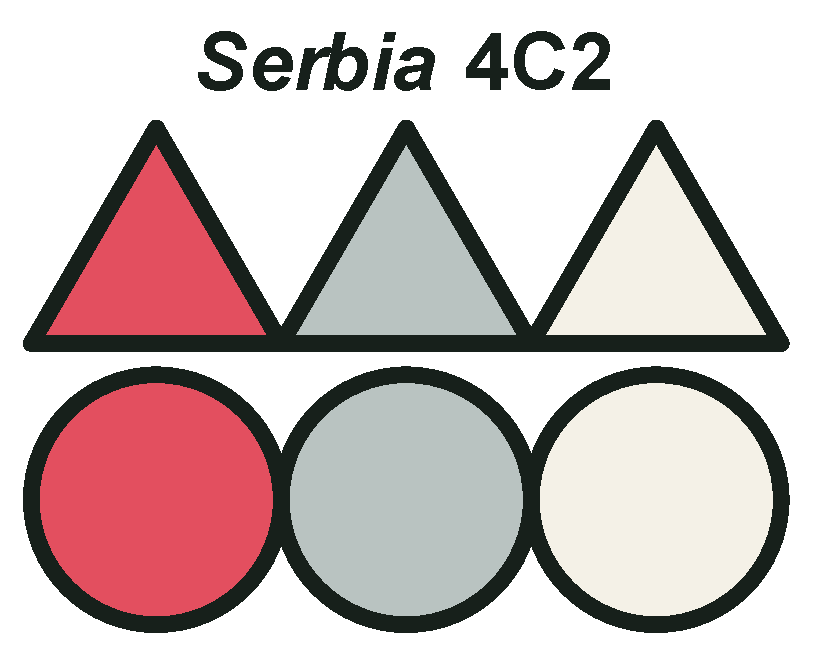
\includegraphics[width=0.64\linewidth]{figures/occupation-zone-display.pdf}
\end{center}

Each Occupation Zone name is followed by three Values. The first is the Garrison Value. The second (a letter) is the Zone’s Alignment Value. The third is the Uprising Modifier (see 7.5).

% Keep the three map-reference illustrations together on printed page 4:
% the Zone display concludes the left column, while the Objective and Neutral
% Chetnik displays occupy the right column.
\columnbreak

\subsection{Objective Displays}\label{sec:5.3}

Each Zone possesses a number of Objective Displays. An Objective Display is simply a rectangle, sub-divided into two boxes of equal size. The left-hand box is meant for the deployment of Yugoslav units — either Partisan or Chetnik, but never both at the same time (this box is printed half in the Partisan color and half in the Chetnik color). The right-hand box is meant for the deployment of Axis units and is colored accordingly. The name of the Display and its terrain type (either city, town, market town, village, or industrial center) is printed across the top of the rectangle. In addition, each Display portrays two Values in the Axis box. These are the Yugoslav Recruitment Value and the Yugoslav Victory Point Value, in that order. The Yugoslav and Axis boxes within a given Objective Display are called corresponding boxes.

\begin{center}
  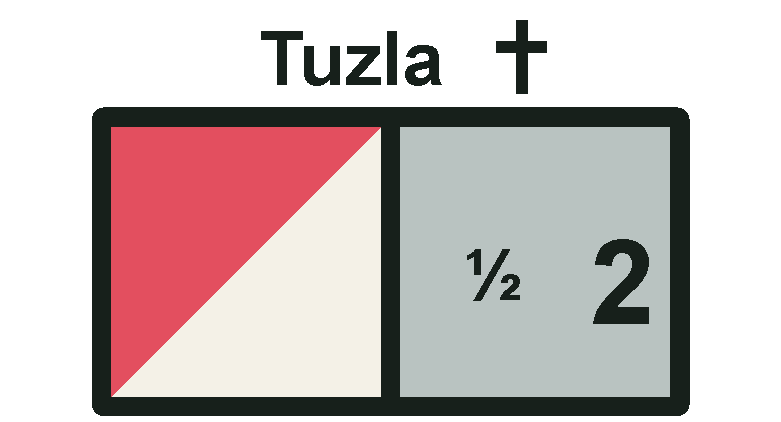
\includegraphics[width=0.60\linewidth]{figures/objective-display.pdf}
\end{center}

\subsection{Neutral Chetnik Boxes}\label{sec:5.4}

All Zones possess a Neutral Chetnik box. During the Chetnik Collaboration Phase, Chetnik units that have become neutral are placed within this box signifying that they are controlled by neither Player (see 7.2).

\begin{center}
  
\includegraphics[width=0.25\linewidth]{figures/neutral-chetnik-box.pdf}
\end{center}
